\chapter{Reti Neurali}
\label{chap:RetiNeurali}

Nel campo dell'apprendimento automatico, o \emph{machine learning}, una rete neurale artificiale  in inglese \emph{Artificial Neural Network} (ANN),  è un modello matematico basato sulla semplificazione delle reti neurali biologiche \cite{samuel1959some}.

Una rete neurale può essere considerata come un sistema dinamico avente la topologia di un grafo orientato con nodi, che modellano i neuroni in un cervello biologico, e archi, che rappresentano le sinapsi (interconnessioni di informazioni).

Ogni connessione può trasmettere un segnale da un neurone artificiale a un altro, i quali sono tipicamente aggregati in strati. Gli stimoli vengono ricevuti da un livello di nodi d'ingresso, detto unità di elaborazione, che elabora il segnale e lo trasmette ad altri neuroni collegati ad esso.

\section{Modello}
\label{sec:modello}

Le reti neurali possono essere viste come semplici modelli matematici che definiscono una funzione $f:X\rightarrow Y$. 

La funzione di rete di un neurone $f(x)$ è definita come una composizione di altre funzioni $g_i(x)$, che possono a loro volta essere scomposte in altre funzioni.

Una rappresentazione ampiamente utilizzata per la descrizione di ANN tradizionali è la \emph{somma ponderata}, mostrata nell'equazione \ref{eq:modellomat}.

\begin{equation}
f(x)=K \bigg( \sum_{i}w_ix_i +b\bigg)
\label{eq:modellomat}
\end{equation}

Ogni segnale in ingresso $x_i$ viene moltiplicato ad un corrispondente peso $w_i$, che assume valore positivo o negativo a seconda che si voglia eccitare o inibire il neurone.  
Il bias $b$ varia secondo la propensione del neurone ad attivarsi, influenzandone l'uscita.
Inoltre viene applicata una funzione predefinita $K$, detta anche \emph{funzione di attivazione}, illustrata nella seguente sezione.

\begin{figure}[htb]
	\centering
	{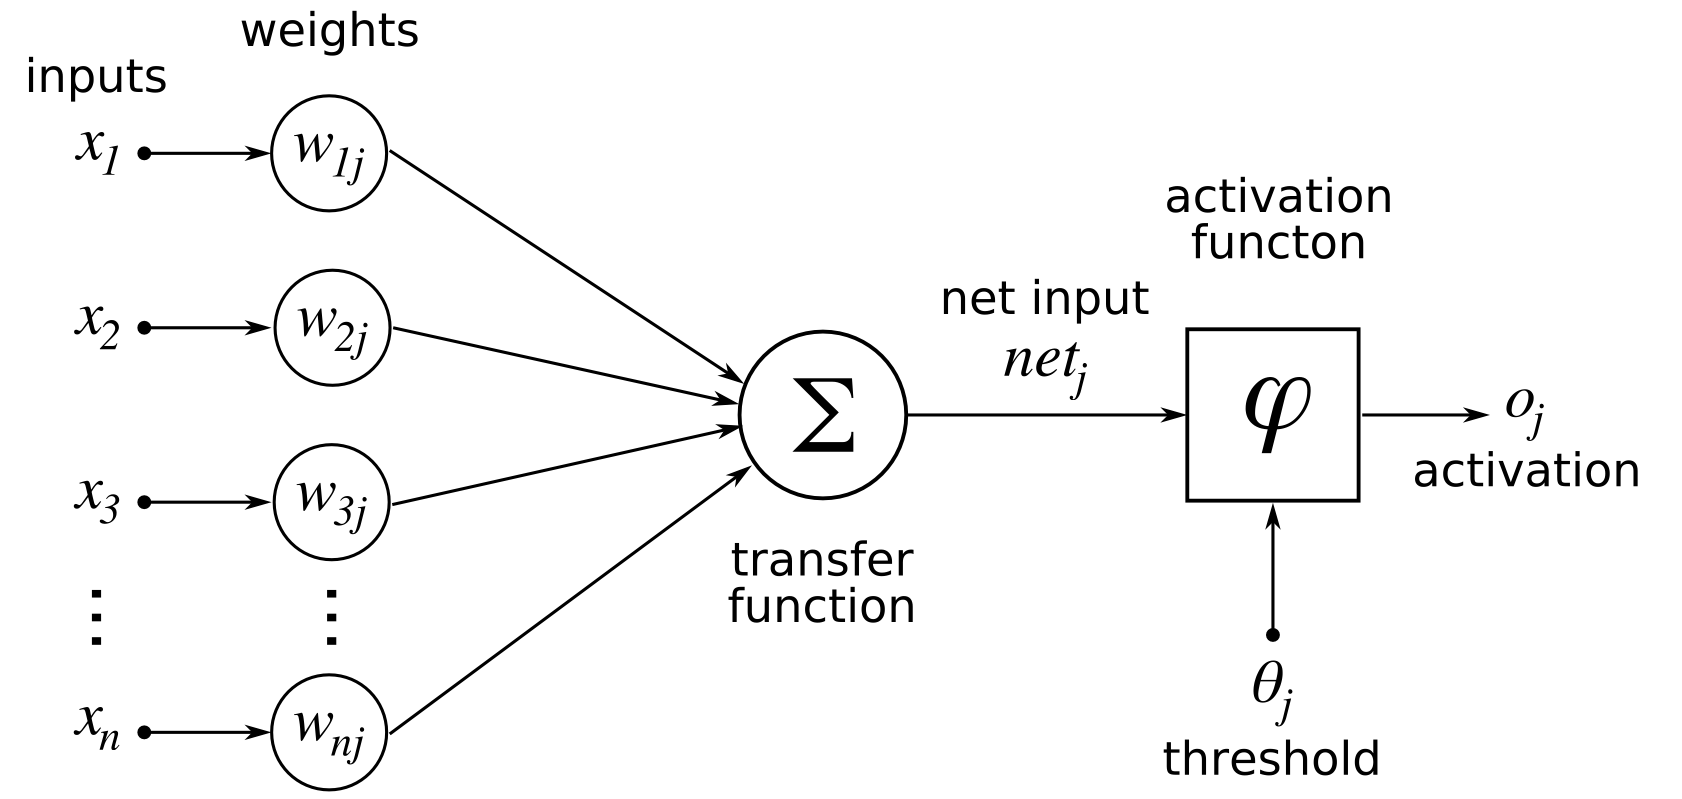
\includegraphics[width=.7\textwidth]{images/ArtificialNeuronModel}} 
	\caption{Artificial Neuron Model}
	\label{fig:Modello matematico di un neurone artificiale}
\end{figure}

\subsection{Funzioni di attivazione}
\label{subsec:fattivazione}
Una funzione di attivazione è una componente fondamentale del modello. Essa consente alla rete di imparare trasformazioni non lineari, in modo da essere in grado di calcolare problemi non banali utilizzando un limitato numero di nodi.

Una delle funzioni più utilizzate è la \emph{sigmoide} $\sigma(x)$, la quale modella la frequenza degli stimoli emessi, da neurone inattivo, $\sigma(x)=0$, a neurone completamente saturo con una frequenza di attivazione massima, $\sigma(x)=1$.

\begin{equation}
\sigma(x) = \frac{1}{1+e^{-x}}
\label{eq:sigmoid}
\end{equation}


Negli ultimi anni è diventata molto popolare la \emph{Rectified Linear Unit} (ReLU) \cite{nair2010rectified,hahnloser2000digital,hahnloser2003permitted,glorot2011deepsparse}, definita dalla seguente equazione:
\begin{equation}
f (x) = \max(0, x)= \begin{cases}
x \quad \mbox{se } x>0\\
0 \quad \mbox{altrimenti}
\end{cases}
\label{eq:relu}
\end{equation}
Questa funzione azzera tutti i valori negativi, mentre ritorna invariati quelli positivi.

Essa viene utilizzata per la sua capacità di accelerare notevolmente la convergenza della discesa del gradiente stocastico, inoltre la sua implementazione risulta semplice ed efficiente.

\begin{figure}[htb]
	\centering
	\subfloat[][\emph{Sigmoide}]
	{\includegraphics[width=.45\textwidth]{images/signmoid2}}
	\quad
	\subfloat[][\emph{ReLU}]
	{\includegraphics[width=.45\textwidth]{images/relu2}} 
	
	\caption{Andamento di due funzioni di attivazione}
	\label{fig:subfig}
\end{figure}


\subsection{Batch normalization}
\label{subsec:normalization}

Per aumentare la stabilità della rete neurale, generalmente viene applicata ad ogni strato una \emph{batch normalization}, la quale normalizza l'uscita di un precedente livello sottraendo il valore medio di un batch e dividendo il risultato per la sua deviazione standard \cite{ioffe2015batch}.

\begin{equation}
	\hat{x}^{(k)}=\frac{x^{(k)}-\mean[x^{(k)}]}{\sqrt{\variance[x^{(k)}]}}
\end{equation}

L'applicazione di questa operazione ad ogni input potrebbe cambiare ciò che il layer può rappresentare. Per questo motivo viene assicurato che la trasformazione inserita nella rete possa rappresentare l'identità, in modo da poter annullare il potenziale effetto della batch normalization, nel caso in cui fosse l'azione ottimale.
Dunque viene prevista l'aggiunta di due parametri --- ``deviazione standard'' $\gamma$ e ``media'' $\beta$ --- che la rete impara assieme ai parametri del modello originale, come mostrato nell'equazione \ref{eq:batchnorm}
\begin{equation}
	y^{(k)}=\gamma^{(k)}\hat{x}^{(k)}+\beta^{(k)}\mbox{.}
	\label{eq:batchnorm}
\end{equation}


\section{Apprendimento}
\label{sec:apprendimento}
Per insegnare alla rete a risolvere un determinato problema, occorre una fase di apprendimento in cui vengono sfruttate una serie di osservazioni per trovare un modello ottimale.

Questo comporta la definizione di una \emph{funzione di costo}, in grado di misurare la distanza tra una soluzione particolare ed una ottimale. 

\subsection{Funzione di costo}
\label{subsec:loss}

Una funzione di costo mappa un evento ad un numero reale, il quale ne rappresenta intuitivamente il ``costo''.

Gli algoritmi di apprendimento cercano di risolvere un problema di ottimizzazione, ovvero la minimizzazione di una certa funzione di perdita. 

Il tipo di problema che si vuole risolvere è una \emph{regressione}, il cui compito è prevedere dei valori reali. Per questo task, è comune calcolare lo scostamento tra la quantità prevista dalla rete $(\hat{Y})$ e i valori osservati $Y$ (ground truth). 
 
L'\emph{errore quadratico medio} (MSE) di uno stimatore misura la media dei quadrati degli errori, e viene calcolato come

\begin{equation}
\mse = \frac{1}{n}\sum_{i=1}^{n}(Y_i-\hat{Y}_i)^2 \mbox{.}
\end{equation}

\subsection{Algoritmi di ottimizzazione}
\label{subsec:optimizer}

Gli algoritmi di ottimizzazione sono necessari per minimizzare il risultato di una determinata funzione obiettivo, la quale dipende dai parametri che il modello deve imparare durante l'addestramento. 

Vengono utilizzate varie strategie e algoritmi di ottimizzazione per aggiornare e calcolare i valori appropriati e ottimali di tale modello, i quali influenzano fortemente l'efficacia del processo di apprendimento.

La tradizionale discesa gradiente, o \emph{Batch Gradient Descent} (GD), calcola il gradiente dell'intero set di dati, eseguendo un solo aggiornamento. Di conseguenza il processo di addestramento può risultare lento e difficile da controllare per i set di dati che sono molto grandi. 

La dimensione dell'aggiornamento è determinata dal tasso di apprendimento $\eta$, in inglese \emph{learning rate}, che garantisce la convergenza al minimo globale, per superfici di errore convesse, e ad un minimo locale, per superfici non convesse. 

\subsubsection{Adagrad}
\label{subsubsec:adagrad}

\emph{Adagrad} è un metodo di apprendimento adattativo che aggiusta il learning rate sulla base dei parametri \cite{duchi2011adaptive} .
In questo algoritmo, la dimensione degli aggiornamenti è grande per parametri associati a caratteristiche poco ricorrenti e piccola per quelli più frequenti. Per questo motivo viene considerato adatto alla gestione di dati sparsi.

Adagrad modifica il tasso di apprendimento generale $\eta$ ad ogni istante di tempo $t$ per ogni parametro $\theta(i)$, sulla base dei gradienti che sono stati calcolati per $\theta(i)$.

Il vantaggio principale di questo metodo è che non è necessario regolare manualmente la frequenza di apprendimento e nella maggior parte delle implementazioni viene usato un valore predefinito --- per esempio \numprint{0,001} --- e lasciato invariato.\\
La principale debolezza consiste nell'accumulo dei ``gradienti quadrati'' nel denominatore, finché ogni termine aggiunto è positivo. Di conseguenza il tasso di apprendimento si riduce fino al punto in cui l'algoritmo non è più in grado di acquisire ulteriori conoscenze. 


\subsubsection{Adam}
\label{subsubsec:adam}

L'\emph{Adaptive Moment Estimation} (Adam) è un altro metodo che calcola i tassi di apprendimento adattivi per ciascun parametro. Oltre a memorizzare una media esponenziale decadente di gradienti quadrati, mantiene anche una media decadente esponenziale dei gradienti passati.

Adam funziona bene se confrontato con altri algoritmi adattativi, poiché converge molto velocemente e la velocità di apprendimento è efficiente.


{\color{blue}
	\subsection{Algoritmo di Backpropagation}
	\label{subsec:backprop}}

\subsection{Paradigmi di apprendimento}
\label{subsec:Paradigmi di apprendimento}

Gli algoritmi di apprendimento sono principalmente suddivisi in due categorie:
\begin{itemize}
	\item[\bfseries supervisionato] --- alla rete viene presentato un training set preparato da un ``insegnante esterno'', composto da coppie significative di valori (input, output atteso).
	
	Quando alla rete neurale viene fornito l'input dall'ambiente, l'insegnante calcola l'output desiderato corrispondente, addestrando la rete mediante un algoritmo (tipicamente quello di back propagation). 
	
	Durante questo procedimento viene calcolo l'errore che la rete commette, dato dalla differenza tra l'output e l'output atteso, necessario per farle comprendere di quanto sbaglia. La rete cerca di minimizzare l'errore commesso, che rappresenta l'azione ottima per l'input corrente, modificando i propri pesi.
	
	In questo moto la rete impara a riconoscere la relazione incognita che lega le variabili di ingresso e uscita, in modo da prevedere il valore di output per qualsiasi valore di ingresso, basandosi solo su una limitata casistica di corrispondenze (coppie input-output).
	
	\item[\bfseries non supervisionato] --- alla rete vengono presentati solo i valori di input, mentre non sono messe a disposizione le informazioni di ritorno dell'ambiente sui valori obiettivo che si vogliono ottenere in risposta o riguardo la correttezza dell'output fornito.
	
	La rete è in grado di individuare da sola pattern, caratteristiche, similarità e regolarità statistiche nei dati di input, acquisendo la capacità di dividerli in cluster rappresentativi che sviluppino delle rappresentazioni interne, senza usare confronti con output noti.
	
	In questo caso, gli algoritmi che modificano i pesi della rete fanno riferimento solo ai dati contenuti nelle variabili di ingresso.
	
	Questo è un tipo di apprendimento autonomo senza controllo esterno sull'errore. È un approccio adatto per ottimizzare le risorse e se non si conoscono a priori i gruppi in cui dividere l'input.
\end{itemize}

\section{Development and test set }
\label{sec:DevelopmentAndTestSet}
Per misurare le prestazioni di una rete neurale dopo la fase di apprendimento, viene creato un test set formato da coppie non utilizzate per il training e validation set.\\
Vengono generalmente definiti: 
\begin{itemize}
	\item Training set --- sul quale viene eseguito l'algoritmo di apprendimento.
	\item Validation set --- viene utilizzato per regolare i parametri, selezionare le features e prendere decisioni per quanto riguarda l'algoritmo di apprendimento.
	\item Test set --- si utilizza per valutare le performance dell'algoritmo, ma non per prendere decisioni su quale algoritmo di apprendimento o parametri utilizzare. 
\end{itemize}

Una volta definiti i set di development e test, ci si concentrerà sul miglioramento delle prestazioni del development set. 

Generalmente la dimensione del test set è un terzo di quella del training. Esso è composto da input critici su cui la risposta della rete deve essere buona. 
Questo funziona bene quando sono messi a disposizione un numero limitato di esempi, ma nell'era dei big data, dove i problemi di apprendimento automatico consistono di più di un miliardo di campioni, la frazione di dati allocati agli insiemi di sviluppo e test è ridotta, nonostante il valore assoluto di esempi sia maggiore.

Vengono utilizzate diverse tecniche statistiche per valutare la bontà di un modello. Normalmente si accetta una rete se sul test set viene mostrato un errore inferiore al \numprin{20-25\%}.


\subsection{Evaluation metric}
\label{subsec:EvaluationMetric}

Le metriche di valutazione spiegano le prestazioni di un modello. Un loro aspetto importante è la capacità di discriminare tra i risultati del modello.
Vengono presi in considerazione diversi tipi di metriche per valutare i modelli. La scelta della metrica dipende completamente dal tipo di modello e dal piano di implementazione. 
\\

I modelli predittivi si distinguo in due principali categorie: si parla di \emph{regressione} quando l'output da prevedere è continuo, o di \emph{classificazione} nel caso in cui l'output sia nominale o binario. Le metriche di valutazione utilizzate in ciascuno di questi modelli sono diverse.

Nei problemi di classificazione, in particolare quella binaria, gli output sono 0 o 1. 
Una \emph{matrice di confusione}, nota anche come matrice di errore, è una tabella $N \times N$, con N corrispondente al numero delle classi, che consente la visualizzazione delle prestazioni di un algoritmo di apprendimento supervisionato. Ogni riga della matrice rappresenta le istanze previste si una classe mentre ciascuna colonna rappresenta le istanze osservate di una classe. 
È dunque possibile estrarre da questa tabella l'\emph{accuratezza} del modello, che consiste nella porzione rispetto al totale delle previsioni corrette, la \emph{precisione}, cioè la porzione dei casi positivi identificati correttamente, e la \emph{recall}, ovvero la porzione dei casi positivi reali correttamente identificati. 

L'individuazione di falsi positivi, falsi negativi, veri positivi e veri negativi, consente un'analisi più dettagliata della semplice proporzione di classificazioni corrette. L'accuratezza infatti non è una metrica attendibile per le prestazioni reali di un classificatore, poiché produrrà risultati fuorvianti se il set di dati non è bilanciato.

L'\emph{errore quadratico medio}(RMSE) è la metrica di valutazione più popolare utilizzata nei problemi di regressione. Questo parametro aiuta a fornire risultati affidabili, mostrando correttamente la grandezza del termine di errore.
La metrica RMSE è definita dalla seguente equazione
\begin{equation}
	\rmse = \sqrt{\frac{\sum_{i=1}^{N}(\mbox{Predicted}_i - \mbox{Actual}_i)^2}{N}} \mbox{.}
	\label{eq:rmse}
\end{equation}

\subsection{Overfitting}
\label{subsec:overfitting}

L'\emph{overfitting} è ``la produzione di un'analisi che corrisponde troppo o esattamente a un particolare insieme di dati, e può quindi non riuscire ad adattare dati aggiuntivi o prevedere in modo affidabile le osservazioni future''.

La rete neurale deve avere capacità di comprensione del modello statistico dei dati, non memorizzare i soli dati del training set. L'essenza di questo problema consiste nell'estrarre inconsapevolmente parte della variazione residua (cioè il rumore) come se quella variazione rappresentasse la sottostante struttura del modello \cite{burnham2003model}.

Per ridurre la possibilità di overfitting esistono diverse tecniche, come la convalida incrociata (cross validation), la regolarizzazione o l'\emph{early stopping}, che consiste nell'utilizzo di un validation set di coppie non usate nel training set per la misurazione dell'errore.

\section{Reti neurali per la classificazione}
\label{sec:classificazione}
La classificazione è la suddivisione di oggetti in insiemi disgiunti secondo un criterio stabilito a priori (etichetta). Ogni oggetto viene rappresentato come un vettore di numeri in modo da poter essere classificato dalla rete neurale, un vettore di feature che contraddistingue univocamente quell'oggetto.\\

Date $N$ classi di appartenenza tra cui discriminare, il vettore di input $x$ possiede $L$ dimensioni delle feature da classificare, il vettore $y$ individua la classe formata da $N$ valori. Il classificatore riceve in input il vettore $x$ e restituisce in uscita il vettore $y$ dove $y_i=1$ se l'oggetto con l'input $x$ appartiene alla classe $i$ e $y_j=0$ per $i\neq j$ per $i,j=1 \dots N$.\\
Questo corrisponde ad una mappatura tra i valori di input e di output, che può essere modellata come una funzione non lineare.

\section{Reti neurali convoluzionali}
\label{sec:cnn}
Una rete neurale convoluzionale, in inglese \emph{Convolutional Neural Network} (CNN), è una classe di reti artificiali avanzate e \emph{feed-forward}, composte da uno o più strati convoluzionali seguiti da una serie di livelli completamente connessi (corrispondenti a quelli tipici di ANN) \cite{kim2014convolutional}. Questa architettura consente alle CNN di sfruttare la struttura 2D dei dati di input.\\

Una convoluzione può essere considerata come una funzione a finestra scorrevole, detta \emph{kernel} o filtro, applicata a una matrice. 
Nelle CNN usiamo le convoluzioni sul livello di input per calcolare l'output. Ciò si traduce in connessioni locali, in cui ogni regione dell'ingresso è collegata a un neurone nell'output. Ogni livello applica filtri diversi, in genere centinaia o migliaia, e combina i loro risultati. 
Durante la fase di addestramento, una CNN impara automaticamente i valori dei suoi filtri in base all'attività che si desidera eseguire. 

Le CNN sono più facili da addestrare rispetto ad altre reti neurali regolari, profonde e feed-forward e hanno molti meno parametri da stimare. Una rete convoluzionale è composta da un input e un livello di output, oltre a più livelli nascosti. Gli strati nascosti consistono tipicamente di livelli convoluzionali, di raggruppamento, o completamente connessi.

Le reti convoluzionali sono adatte per elaborare dati visivi e altri dati bidimensionali, ed hanno mostrato ottimi risultati nel riconoscimento di immagini o nella manipolazione del linguaggio naturale \cite{manning1999foundations,FIXME}.
In quest'ultimo caso, l'input sono frasi o documenti rappresentati come una matrice. Ogni riga della matrice corrisponde a un token, in genere una parola. Tipicamente, questi vettori sono dei word embeddings (rappresentazioni a bassa dimensione) come word2vec \cite{mikolov2013distributed} o GloVe \cite{pennington2014glove}, ma potrebbero anche essere vettori unici che indicizzano la parola in un vocabolario. 

Nel \emph{Natural Language Processing} (NLP) utilizziamo filtri che scorrono su righe complete della matrice (parole), pertanto, la loro ``larghezza'' è solitamente uguale alla quella della matrice di input. L'altezza, o la dimensione della regione, può variare, ma le finestre tipicamente scorrono su 2-5 parole per volta. 

Risulta che le CNN applicate ai problemi di NLP funzionino abbastanza bene, un esempio è il modello \emph{Bag of Words} che è stato l'approccio standard per anni e ha portato a risultati piuttosto buoni.
